%! Author = Wiktor Rostkowski, Mateusz Budzisz
%! Date = 29/04/2024

\chapter{Testy}
\label{ch:testy}

\section{Testy jednostkowe}
\label{sec:testy-jednostkowe}
W naszej pracy inżynierskiej zastosowaliśmy GitHub Actions do automatyzacji testów jednostkowych(opisane \pageref{sec:github-actions} ), które przeprowadziliśmy dla różnych komponentów naszego projektu.
Testy jednostkowe były kluczowym elementem, zapewniającym jakość~i~niezawodność naszego oprogramowania. 
W sumie przeprowadziliśmy 638 testów, obejmujących frontend, backend oraz dokumentację.\newline

\indent W ramach projektu frontend wykonaliśmy 151 testów jednostkowych, koncentrując się na każdym komponencie aplikacji. Testy te obejmowały funkcjonalności poszczególnych 
komponentów, sprawdzając ich poprawne renderowanie, interakcje użytkownika oraz walidację danych. Głównym celem było zapewnienie, że każdy komponent działa zgodnie~z~założeniami~i~spełnia swoje funkcje.\newline

\indent Dla backendu obejmował 159 testów jednostkowych, które dotyczyły logiki biznesowej, operacji na danych oraz interakcji~z~bazą danych. 
Testowaliśmy funkcje oraz metody, aby upewnić się, że zwracają one poprawne wyniki~w~różnych scenariuszach. Dodatkowo sprawdzaliśmy poprawność integracji wszystkich zależności~i~usług zewnętrznych.\newline

\indent Na potrzeby projektu prowadząc dokumentacje przeprowadziliśmy 328 testów jednostkowych, które miały na celu weryfikację poprawności oraz kompletności dokumentacji technicznej~i~użytkowej.
 Sprawdzaliśmy, czy wszystkie przykłady kodu działają poprawnie~i~czy dokumentacja jest aktualna~w~stosunku do bieżącego stanu projektu. Testy te były kluczowe dla zapewnienia, że dokumentacja 
 jest pomocna~i~dokładna, wspierając użytkowników~i~deweloperów~w~korzystaniu~z~naszego systemu.\newline

 \indent Podsumowując, przeprowadzenie łącznie 638 testów jednostkowych pozwoliło nam na dogłębne sprawdzenie działania naszej aplikacji na każdym etapie naszej pracy. 
Wykorzystanie GitHub Actions do automatyzacji testów zapewniło efektywność~i~powtarzalność procesu testowania, co jest kluczowe dla utrzymania wysokiej jakości oprogramowania. 
Dzięki temu podejściu jesteśmy pewni, że nasza aplikacja jest dobrze przetestowana~i~gotowa do wdrożenia.\newline

\begin{figure}[H]
    \centering
    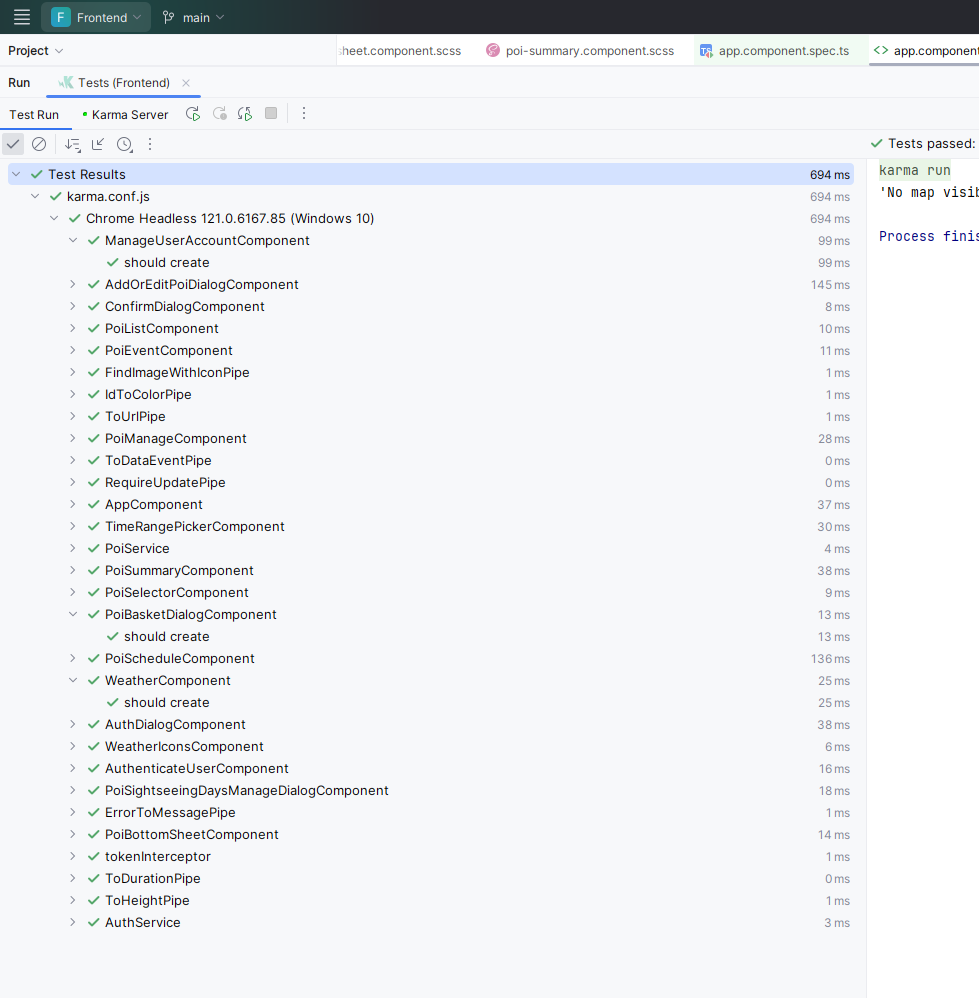
\includegraphics[width=1\textwidth]{attachments/testfrontend}
    \caption{Testy jednostkowe Frontend}
    \label{fig:testfronted}
\end{figure}

\section{Testy wydajnościowe}
\label{sec:testy-wydajnosciowe}

W ramach naszej pracy inżynierskiej wykonaliśmy testy wydajności~za~pomocą narzędzia Lighthouse, aby ocenić~i~poprawić wydajność naszej aplikacji internetowej. \newline
Lighthouse jest narzędziem open-source opracowanym przez Google, które automatycznie ocenia strony internetowe pod kątem wydajności, dostępności, najlepszych praktyk~i~SEO. \newline
Przeprowadziliśmy testy zarówno dla wersji mobilnej, jak~i~desktopowej naszej aplikacji. \newline
Zdecydowaliśmy się na Lighthouse ze względu na jego wszechstronność~i~precyzję~w~ocenie kluczowych aspektów wydajnościowych.  \newline
Narzędzie to jest szeroko stosowane~w~branży~i~dostarcza szczegółowych raportów, które pomagają zidentyfikować obszary wymagające optymalizacji. \newline
\begin{figure}[H]
    \centering
    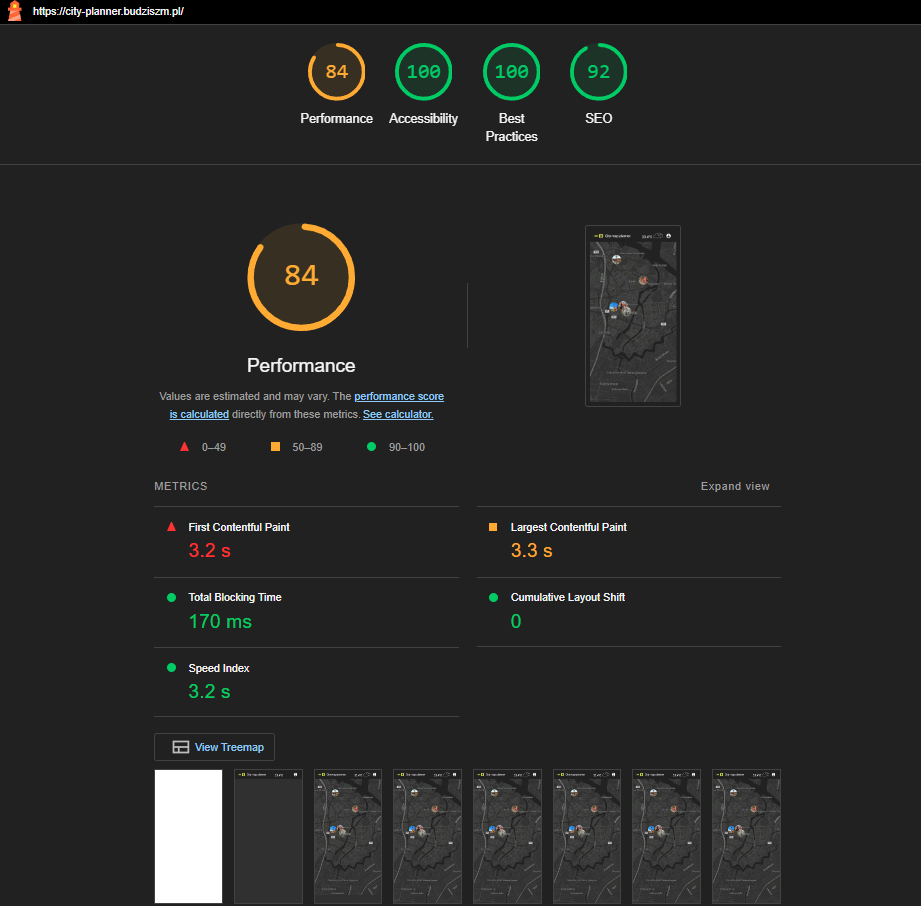
\includegraphics[width=1\textwidth]{attachments/lighthouse-mobile}
    \caption{Widok testu lighthouse mobile}
    \label{fig:testy-lighthouse-mobile}
    \end{figure}

    \begin{figure}[H]
        \centering
        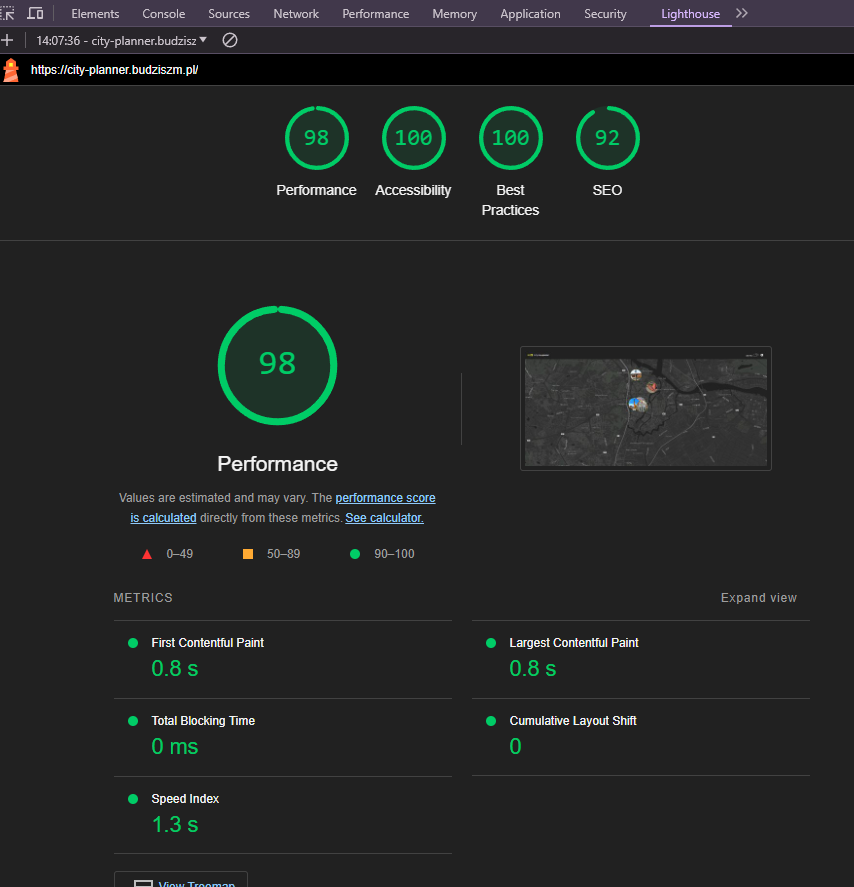
\includegraphics[width=1\textwidth]{attachments/lighthouse}
        \caption{Widok testu lighthouse komputer}
        \label{fig:testy-lighthouse-desktop}
        \end{figure}
\section{Testy funkcjonalne}
\label{sec:testy-funkcjonalne}

Na koniec każdego przyrostu projektu przeprowadzaliśmy testy funkcjonalne. Za te testy odpowiadała wyznaczona osoba, która nie brała udziału~w~implementacji danego przyrostu. 
Testy funkcjonalne miały na celu weryfikację działania konkretnej funkcjonalności związanej~z~danym zadaniem. \newline
Dla zadań bezpośrednio związanych~z~implementacją user story lub wymagania niefunkcjonalnego, testy przeprowadzano zgodnie~z~ustalonymi kryteriami akceptacji. \newline
Jeśli podczas testów wykryto, że wprowadzone zmiany mają negatywny wpływ na inne obszary projektu, zadanie było zwracane~w~celu dokonania niezbędnych poprawek.\newline
\indent Jednym~z~kluczowych aspektów naszej aplikacji było zapewnienie jej dostępności dla wszystkich użytkowników,~w~tym dla osób~z~niepełnosprawnościami.
 Aby ocenić poziom dostępności aplikacji, przeprowadzono test~za~pomocą narzędzia Lighthouse.

 Audyt dostępności obejmował ocenę różnych elementów strony, takich jak 
 struktura nagłówków, kontrast kolorów, alternatywne opisy obrazków, możliwość nawigacji~za~pomocą klawiatury, 
 obsługa technologii asystujących, oraz zgodność~z~wytycznymi WCAG (Web Content Accessibility Guidelines). \newline
 \indent Wynik uzyskany~w~kategorii dostępności to 100, co oznacza, że aplikacja internetowa spełnia wszystkie kryteria dostępności oceniane przez Lighthouse.
 Dzięki zastosowaniu najlepszych praktyk~i~spełnieniu wytycznych WCAG, aplikacja jest przyjazna dla szerokiego grona użytkowników,~w~tym osób~z~niepełnosprawnościami.
\begin{figure}[H]
    \centering
    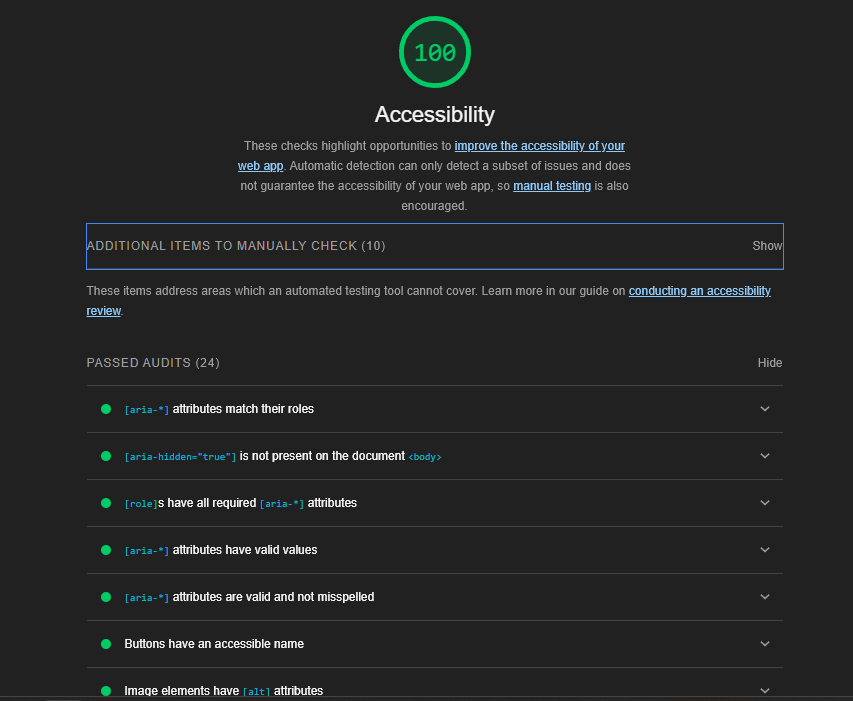
\includegraphics[width=1\textwidth]{attachments/testy-dostepnosci}
    \caption{Widok testu dostępności dla naszej aplikacji}
    \label{fig:testy-dostepnosci-zdjecie}
    \end{figure}


\section{Scenariusze testowe}
\label{sec:scenariusze-testowe}

W niniejszym rozdziale przedstawiono szczegółowe scenariusze testowe, które zostały przeprowadzone podczas realizacji 
poszczególnych przyrostów~w~ramach projektu. Celem tych testów było zapewnienie wysokiej jakości oraz funkcjonalności 
rozwijanej aplikacji, a także weryfikacja zgodności implementacji~z~założeniami projektowymi~i~wymaganiami użytkowników.

\begin{testowanie}[label={tab:requirements:testnowy1},caption={Scenariusz testowy: Logowania użytkownika}]
    \name{Sprawdzenie pracy widoku logowania}
    \descr{Testowanie logowania}
    \type{WO1,F24}
    \env{Włączona strona główna aplikacji}
    \test{}
    \testz{1. Otwórz menu logowania.}{Menu logowania jest wyświetlane.}
    \testy{2. Wprowadź poprawne dane logowania.}{Użytkownik jest zalogowany.}
    \result{Sukces}
    \testX{}
    \testXz{1. Otwórz menu logowania.}{Strona logowania jest wyświetlane.}
    \testXy{2. Wprowadź niepoprawne dane logowania.}{Pojawia się komunikat o błędzie.}
    \resultX{Niepowodzenie}
\end{testowanie}

\begin{testowanie}[label={tab:requirements:testnowy2},caption={Scenariusz testowy: Zarzadzania POI}]
    \name{Sprawdzenie możliwości zarządzania POI}
    \descr{Sprawdzenie możliwości czy jest możliwość zarządzania POI bez uprawnień administratora}
    \type{FO4}
    \env{Włączona strona główna aplikacji}
    \test{}
    \testz{1. Zaloguj się jako zwykły użytkownik}{Użytkownik zalogowany}
    \testy{2. Włącz stronę do zarządzania POI}{ Otwarcie panelu zarządzania}
    \result{Niepowodzenie, brak możliwości wczytania informacji}
    \testX{}
    \testXz{1. Zaloguj się jako administrator}{Administrator zalogowany}
    \testXy{2. Włącz stronę do zarządzania POI}{ Otwarcie panelu zarządzania}
    \resultX{ Panel zarządzania POI załadowany prawidłowo}
\end{testowanie}

\begin{testowanie}[label={tab:requirements:testnowy3},caption={Scenariusz testowy: Test mapy}]
    \name{Test mapy}
    \descr{Sprawdzenie funkcjonowania mapy}
    \type{F01, IO3,IO4}
    \env{Włączona strona główna aplikacji}
    \test{}
    \testz{1. Przesuwaj na mapie~w~różne strony}{ Mapa zmienia położenie względem ustalonego przeciągnięcia}
    \result{Mapa przesuwa się zgodnie~z~żądaniem}
\end{testowanie}

\begin{testowanie}[label={tab:requirements:testnowy4},caption={Scenariusz testowy: Rejestracja użytkownika}]
    \name{Sprawdzenie funkcjonowania rejestracji użytkownika}
    \descr{Testowanie Rejestracji użytkowników}
    \type{WO6}
    \env{Włączona strona główna aplikacji,~z~otwartym menu użytkownika}
    \test{}
    \testz{1. Otwórz menu użytkownika.}{Menu rejestracji jest wyświetlane.}
    \testy{2. Wprowadź poprawne dane do rejestracji.}{Rejestracja wymusza akceptacja linku}
    \testy{3. Kliknij  link otrzymany na maila.}{Rejestracja powiodła się pomyślnie.}
    \testy{4. Wykonaj czynności~z~testu logowania.}{Logowanie wykonało się pomyślnie.}
    \result{Sukces - użytkownik zalogowany}
    \testX{}
    \testXz{1. Otwórz menu użytkownika.}{Menu rejestracji jest wyświetlane.}
    \testXy{2. Wprowadź poprawne dane do rejestracji.}{Rejestracja wymusza akceptacja linku}
    \testXy{3. Wykonaj czynności~z~testu logowania, \newline wykorzystując dane~z~rejestracji bez akceptacji linku}{Logowanie nie wykonało się pomyślnie.}
    \resultX{Niepowodzenie logowania}
\end{testowanie}

\begin{testowanie}[label={tab:requirements:testnowy5},caption={Scenariusz testowy: Test POI}]
    \name{Test działania znacznika POI}
    \descr{Sprawdzenie funkcjonowania punktów POI na mapie}
    \type{FO5}
    \env{Włączona strona główna aplikacji}
    \test{}
    \testz{1. Kliknij POI dostępne na mapie}{ POI wyświetla się od razu po kliknięciu}
    \result{POI wyświetla się~z~wszystkimi informacjami}
    \testX{}
    \testXz{1. Kliknij na mapie dowolny element}{ Brak żadnej reakcji }
    \resultX{Nie wykonała się żadna akcja}
\end{testowanie}

\begin{testowanie}[label={tab:requirements:testnowy6},caption={Scenariusz testowy: Test koszyk POI}]
    \name{Test działania koszyka}
    \descr{Sprawdzenie funkcjonowania koszyka}
    \type{FO19}
    \env{Włączona strona główna aplikacji}
    \test{}
    \testz{1. Kliknij POI dostępne na mapie}{ POI wyświetla się od razu po kliknięciu}
    \testz{2. Kliknij ikone koszyk plus na karcie POI}{ POI dodaje się do koszyka koszyk wyświetla się na pasku nawigacji. \newline ikona koszyka~w~poi zmieniła się na minus koszyk}
    \testz{3. Kliknij Koszyk na pasku nawigacji}{ Wyświetla się koszyk~z~wybranym wcześniej POI}
    \result{W koszyku wyświetla się POI~z~możliwością jego usuniecia}
    \testX{}
    \testXz{1. Kliknij POI dostępne na mapie}{ POI wyświetla się od razu po kliknięciu}
    \testXz{2. Kliknij ikone koszyk plus na karcie POI}{ POI dodaje się do koszyka koszyk wyświetla się na pasku nawigacji. \newline ikona koszyka~w~poi zmieniła się na minus koszyk}
    \testXz{3. Kliknij ikone koszyk minus POI}{ Koszyk zniknął}
    \resultX{Nie ma możliwości klikniecia~w~koszyk,gdyż nie ma żadnego POI}
\end{testowanie}

\begin{testowanie}[label={tab:requirements:testnowy7},caption={Scenariusz testowy: Test kalendarz planowania}]
    \name{Test działania kalendarza}
    \descr{Sprawdzenie funkcjonowania planera podróży}
    \type{FO14}
    \env{Wykonaj Test działania koszyka przypadek I dwukronie}
    \test{}
    \testz{1. W koszyku kliknij  przekierowanie do planera}{ Otwiera się kalendarz~z~wcześniej zaznaczonymi POI}
    \testz{2. W kalendarzu przeciągnij POI na jakikolwiek okres czasowy, który jest zaznaczony~w~tym samym kolorze co POI }{ Udało się przeciągnąć POI na okres czasowy}
    \testz{3. W ciągnąć~za~dolny element POI skróć jego czas występowania~w~kalendarzu }{ Udało się zmodyfikować czas zaplanowanego POI}
    \result{W POI występuje na kalendarzu}
    \testX{}
    \testXz{1. W koszyku kliknij  przekierowanie do planera}{ Otwiera się kalendarz~z~wcześniej zaznaczonymi POI}
    \testXz{2. W kalendarzu przeciągnij POI na jakikolwiek okres czasowy, który jest nie jest~w~tym samym kolorze co POI}{Nie udało się przeciągnąć POI na okres czasowy, POI wróciło na element startowy}
    \resultX{Nie ma możliwości przeciągnięcia POI na okres czasowy,~w~którym POI jest niedostępne lub użytkownik nie ma czasu}
\end{testowanie}

\begin{testowanie}[label={tab:requirements:testnowy8},caption={Scenariusz testowy: Test widoku podsumowania planowania}]
    \name{Test działania podsumowania~i~planowania trasy}
    \descr{Sprawdzenie funkcjonowania planera podróży}
    \type{FO13, F10, F27}
    \env{Wykonaj Test działania  kalendarza przypadek I}
    \test{}
    \testz{1. W kalendarzu kliknij  przekierowanie do podsumowania podróży}{ Otwiera się podsumowanie~z~wcześniej zaznaczonymi POI~w~danym okresie czasowym}
    \result{ W tym widoku widać przeznaczone wszystkie poprzednie informacje. \newline
        Widać okres czasowy zaznaczony na czas zwiedzania atrakcji~w~tym pogodę na ten okres czasowy.
        Jest przedstawiona rekomendowana pogoda dotycząca zwiedzenia tej atrakcji.
        Jako podsumowanie widać opis tej atrakcji.
        }
        \testXz{1. W kalendarzu kliknij  przekierowanie do podsumowania podróży}{ Otwiera się podsumowanie~z~wcześniej zaznaczonymi POI~w~danym okresie czasowym}
        \testXz{2. W podsumowaniu kliknij atrakcje numer dwa}{ Zaczyna się przeszukiwanie najszybciej drogi~z~jednego do drugiego POI }
    \resultX{Widok przestawia  mapę~z~trasą podróży}
\end{testowanie}



\begin{testowanie}[label={tab:requirements:testnowy2},caption={Scenariusz testowy: Zarzadzania POI~z~wykorzystaniem ChatGPT}]
    \name{Sprawdzenie możliwości zarządzania POI}
    \descr{Sprawdzenie możliwości aktualizowanie godzin otwarcia}
    \type{IO7}
    \env{Włączona strona zarządzania POI~z~użytkownikiem o uprawnieniach administratora}
    \test{}
    \testz{1. Kliknij przycisk edycji POI}{Edytor POI się otwiera}
    \testy{2. Włącz stronę do zarządzania POI}{ Otwarcie panelu zarządzania}
    \testy{3. Kliknij zaczytanie informacji na podstawie AI}{ Ładowanie danych}
    \result{Niepowodzenie, brak możliwości wczytania informacji}
    \testX{}
    \testy{1. Włącz stronę do zarządzania POI}{ Otwarcie panelu zarządzania}
    \testy{2. Kliknij zaczytanie informacji na podstawie AI}{ Ładowanie danych}
    \resultX{ Godziny wszystkich atrakcji załadowały}
\end{testowanie}


